


We provide an in-depth analysis of the Uhlmann transformation algorithm in the purified sample access model.
The main challenge here, compared to the purified query access model, is to prepare a unitary that encodes $\tr_{\sA'}\big[\ketbra{\sigma}{\rho}^{\sA'\sB}\big]$ directly from given states $\ket{\rho}^{\hat{\sA}\hat{\sB}}$ and $\ket{\sigma}^{\hat{\sA}\hat{\sB}}$, rather than from unitaries $U_\rho^{\hat{\sA}\hat{\sB}}$ and $U_\sigma^{\hat{\sA}\hat{\sB}}$ that generate them.
To this end, we propose a method inspired by the density matrix exponentiation.


Let $\sH$ be a two-qubit system, and let $\cP_{\ket{0}\ket{\sigma}}^{\bC\rarr\sH\hat{\sA}\hat{\sB}}$ be a state-preparation channel given by $\cP_{\ket{0}\ket{\sigma}}^{\bC\rarr\sH\hat{\sA}\hat{\sB}} = \ketbra{0^2}{0^2}^\sH \otimes \ketbra{\sigma}{\sigma}^{\hat{\sA}\hat{\sB}}$.
The following is a formal statement of \Cref{infthm:uhlmenn purif sample}.





\begin{theorem}[Uhlmann transformation algorithm in the purified sample access model]
\label{thm:algorithm Uhlmann}
Let $\delta \in (0, 1)$ and $\chi \in \{\diamond, \tF\}$. Then, the quantum sample algorithm $\mathtt{UhlmannPurifiedSample}$ given by \Cref{alg:Uhl purif sample} satisfies the following.

A quantum channel $\cJ_\diamond^{\sB\sH\hat{\sA}\hat{\sB}}$ given by $\cJ_\diamond^{\sB\sH\hat{\sA}\hat{\sB}} = \mathtt{UhlmannPurifiedSample}(\ket{\rho}^{\hat{\sA}\hat{\sB}}, \ket{\sigma}^{\hat{\sA}\hat{\sB}}; \delta, \diamond)$,
satisfies that
\begin{equation}
    \f{1}{2}\big\|\cJ_\diamond^{\sB\sH\hat{\sA}\hat{\sB}} \circ\cP_{\ket{0}\ket{\sigma}}^{\bC\rarr\sH\hat{\sA}\hat{\sB}} - \cU_{\rm ideal}^{\sB\sH\hat{\sA}\hat{\sB}}\circ\cP_{\ket{0}\ket{\sigma}}^{\bC\rarr\sH\hat{\sA}\hat{\sB}}\big\|_\diamond \leq \delta,
\end{equation}
where $U_{\rm ideal}^{\sB\sH\hat{\sA}\hat{\sB}}$ is an exact block-encoding unitary of $\ketbra{\rho}{\sigma}^{\hat{\sA}\hat{\sB}} \otimes V^\sB$ and $V^\sB$ is the Uhlmann partial isometry.
The algorithm uses $w_\diamond = \cO\Big(\f{1}{\delta s_{\rm min}^2}\big(\log{\big(\f{1}{\delta}\big)}\big)^2\Big)$ samples of $\ket{\rho}^{\hat{\sA}\hat{\sB}}$ and $\ket{\sigma}^{\hat{\sA}\hat{\sB}}$.

Moreover, a quantum channel $\cJ_{\tF}^{\sB\sH\hat{\sA}\hat{\sB}}$ given by $\cJ_{\tF}^{\sB\sH\hat{\sA}\hat{\sB}} = \mathtt{UhlmannPurifiedSample}(\ket{\rho}^{\hat{\sA}\hat{\sB}}, \ket{\sigma}^{\hat{\sA}\hat{\sB}}; \delta, \tF)$,
satisfies that
\begin{align}
        \rF\big(\cT^\sB(\ketbra{\rho}{\rho}^{\sA\sB}), \ket{\sigma}^{\sA\sB}) \geq \rF(\rho^\sA, \sigma^\sA) - \delta,
\end{align}
where $\cT^\sB = \tr_{\sH\hat{\sA}\hat{\sB}}\circ\cJ_{\tF}^{\sB\sH\hat{\sA}\hat{\sB}}\circ\cP_{\ket{0}\ket{\sigma}}^{\bC\rarr\sH\hat{\sA}\hat{\sB}}$.
The algorithm uses $w_{\tF} = \cO\Big(\f{1}{\delta}\min\big\{\f{1}{s_{\rm min}^2}, \f{r^2}{\delta^2}\big\}\big(\log{\big(\f{1}{\delta}\big)}\big)^2\Big)$ samples of $\ket{\rho}^{\hat{\sA}\hat{\sB}}$ and $\ket{\sigma}^{\hat{\sA}\hat{\sB}}$.

In both cases, the quantum circuit for implementing the algorithm consists of $\cO\big(w_\chi \log{(d_\sA d_\sB)}\big)$ one- and two-qubit gates, and $\cO\big(\log{(d_\sA d_\sB)}\big)$ qubits suffice at any one time.
\end{theorem}




%===================================================================================================================================================================================================================================

\begin{algorithm}[h]
\caption{Uhlmann transformation algorithm in the purified sample model \\ \parbox{\linewidth}{\centering $\mathtt{UhlmannPurifiedSample}(\ket{\rho}^{\hat{\sA}\hat{\sB}}, \ket{\sigma}^{\hat{\sA}\hat{\sB}}; \delta, \chi)$ (In Theorem~\ref{thm:algorithm Uhlmann})}}
\label{alg:Uhl purif sample}
\SetKwInput{KwInput}{Input}
\SetKwInput{KwOutput}{Output}
\SetKwInput{KwParameters}{Parameters}
\SetKwComment{Comment}{$\triangleright$\ }{}
\SetCommentSty{textnormal}

\SetAlgoNoEnd
\SetAlgoNoLine
\KwInput{Two pure quantum state $\ket{\rho}^{\hat{\sA}\hat{\sB}}$ and $\ket{\sigma}^{\hat{\sA}\hat{\sB}}$.}
\KwParameters{$\delta \in (0, 1)$ and $\chi \in \{\diamond, \tF\}$.}
\KwOutput{Quantum channel $\cJ^{\sB\sH\hat{\sA}\hat{\sB}}$.}
\SetAlgoLined

Prepare a quantum state $\Upsilon^{\sC_2\sC_3\sA_1\sB_1\sB_2}$ (Eq.~\eqref{inteq:64}) by running the circuit in \Cref{fig:upsilon circuit} with $\ket{\rho}^{\sA_1\sB_1}$ and $\ket{\sigma}^{\sA_2\sB_2}$. \\
\If{$\chi = \diamond$}{
  Set $\delta_1 \gets (\delta/6)^2$ and $\beta \gets 2s_{\rm min}/\pi$. \\
}
\ElseIf{$\chi = \tF$}{
  Set $\delta_1 \gets \delta/8$ and $\beta \gets \f{1}{\pi}\max\{2s_{\rm min}, \delta_1/r\}$. \\
}
Set $u$ to be the minimum odd integer satisfying $u \geq \big\lceil\f{8e}{\beta}\log{(2/\delta_1)}\big\rceil$. \\
Set $\delta_2 \gets \delta/(2u)$. \\
Set $\cF^{\sC\hat{\sA}\hat{\sB}\sB} \gets \mathtt{DMESUB}(\Upsilon^{\sC_2\sC_3\sA_1\sB_1\sB_2}; \delta_2, t=2)$ and $\cF_{\rm inv}^{\sC\hat{\sA}\hat{\sB}\sB} \gets \mathtt{DMESUB}^\dag(\Upsilon^{\sC_2\sC_3\sA_1\sB_1\sB_2}; \delta_2, t=2)$ (Proposition~\ref{prevthm:DME variant}). \\
Set $\cG^{\sC\hat{\sA}\hat{\sB}\sB} \gets \cX^\sC\circ\cF^{\sC\hat{\sA}\hat{\sB}\sB}$ and $\cG_{\rm inv}^{\sC\hat{\sA}\hat{\sB}\sB} \gets \cF_{\rm inv}^{\sC\hat{\sA}\hat{\sB}\sB}\circ\cX^\sC$, where $\cX^\sC(\cdot) = X^\sC(\cdot)X^\sC$ and $X^\sC$ is the one-qubit Pauli-$X$ gate on $\sC$. \\
Set $\cJ^{\sB\sH\hat{\sA}\hat{\sB}} \gets \mathtt{QSVTSIGN}(\cG^{\sC\hat{\sA}\hat{\sB}\sB}, \cG_{\rm inv}^{\sC\hat{\sA}\hat{\sB}\sB}; \delta_1, \beta)$ (Proposition~\ref{prop:FPAA general}). \\
Return $\cJ^{\sB\sH\hat{\sA}\hat{\sB}}$.
\end{algorithm}


At a high level, \Cref{alg:Uhl purif sample} proceeds in three steps:
\begin{align}
\ket{\rho}^{\sA_1\sB_1}, \ket{\sigma}^{\sA_2\sB_2}
&\hspace{0.6pc}\overset{1. \, \text{Fig.~\ref{fig:upsilon circuit}}}{\longrightarrow}\hspace{0.5pc}
\Upsilon^{\sC_2\sC_3\sA_1\sB_1\sB_2} \\
&\hspace{0.3pc}\overset{2. \, \mathtt{DMESUB}}{\longrightarrow}\hspace{0.5pc}
e^{i(\ketbra{1}{0}^\sC \otimes L^{\hat{\sA}\hat{\sB}\sB} + \ketbra{0}{1}^\sC\otimes (L^{\hat{\sA}\hat{\sB}\sB})^\dag)} \\
&\hspace{0.1pc}\overset{3. \, \mathtt{QSVTSIGN}}{\longrightarrow}\hspace{0.5pc}
\begin{pmatrix}
    \hspace*{1.5mm} \ketbra{\rho}{\sigma}^{\hat{\sA}\hat{\sB}} \otimes V^\sB & \hspace*{0mm} * \hspace*{3mm} \\
    \hspace*{2mm} * & \hspace{0mm} * \hspace*{3mm}
\end{pmatrix},
\end{align}
where $L^{\hat{\sA}\hat{\sB}\sB} = \ketbra{\rho}{\sigma}^{\hat{\sA}\hat{\sB}}\otimes\tr_{\sA'}\big[\ketbra{\sigma}{\rho}^{\sA'\sB}\big]$ and $V^\sB$ is the Uhlmann partial isometry.
The number of samples of $\ket{\rho}^{\hat{\sA}\hat{\sB}}$ and $\ket{\sigma}^{\hat{\sA}\hat{\sB}}$ required in step~1 is $\cO(1)$, and in step~2, the number of samples of $\Upsilon$ is $\cO(1/\delta)$ by \Cref{prevthm:DME variant}. In step~3, the number of uses of $e^{i(\ketbra{1}{0} \otimes L + \ketbra{0}{1}\otimes L^\dag)}$ is $\cO(\log(1/\delta)/\beta)$ by \Cref{prop:FPAA general}.  
Thus, the total sample complexity of $\ket{\rho}^{\hat{\sA}\hat{\sB}}$ and $\ket{\sigma}^{\hat{\sA}\hat{\sB}}$ for \Cref{alg:Uhl purif sample} is given by the product of these, namely, $\cO\big(\log(1/\delta)/(\beta\delta)\big)$.  
Note that the parameters $\delta$ and $\beta$ are chosen so that the overall approximation error remains within $\delta$, thereby demonstrating our statement in Theorem~\ref{thm:algorithm Uhlmann}.




Note that, in \Cref{alg:Uhl purif sample}, $\mathtt{QSVTSIGN}$ takes a quantum channel $\cG$ (and $\cG_{\rm inv}$) as an input, instead of a unitary $W$ (and $W^\dag$).
This represents that in the quantum circuit for $\mathtt{QSVTSIGN}$, every access to $W$ is replaced by an access to $\cG$. 
As a result, the output of $\mathtt{QSVTSIGN}$ is not a unitary $\til{W}$ whose top-left block approximates the sign function, but rather a quantum channel $\cJ$.
We need to evaluate the distance between the actual output channel $\cJ$ and the desired unitary channel $\til{\cW}$.
The error in approximating $\cW$ by $\cG$ accumulates proportionally to the number of repetitions $u$ in $\mathtt{QSVTSIGN}$, resulting in the error in approximating $\til{\cW}$ by $\cJ$.
To keep the final error sufficiently small, the initial error of $\cG$ in approximating $\cW$ is pre-scaled by $1/u$.
For this reason, $u$ appears in the denominator of the assignment in line~7 of \Cref{alg:Uhl purif sample}.


%===================================================================================================================================================================================================================================






The additional factor $\ketbra{\rho}{\sigma}^{\hat{\sA}\hat{\sB}}$ appears in the top-left block of $U_{\rm ideal}^{\sB\sH\hat{\sA}\hat{\sB}}$ in Theorem~\ref{thm:algorithm Uhlmann}.
This does not cause any issues, since we do not operate on system $\sA$.
To see this, we fix the input state to $\ket{\rho}^{\sA\sB}$ and observe that 
\begin{align}
    |\bra{\sigma}^{\sA\sB}\bra{0}^\sH\bra{\rho}^{\hat{\sA}\hat{\sB}}U_{\rm ideal}^{\sB\sH\hat{\sA}\hat{\sB}}\ket{\rho}^{\sA\sB}\ket{0}^\sH\ket{\sigma}^{\hat{\sA}\hat{\sB}}|
    &= |\bra{\sigma}^{\sA\sB}\bra{0}^\sH \bra{\rho}^{\hat{\sA}\hat{\sB}}V^\sB\ket{\rho}^{\sA\sB}\ket{0}^\sH\ket{\rho}^{\hat{\sA}\hat{\sB}}| \\
    &=  \rF(\rho^\sA, \sigma^\sA),
\end{align} 
where $V^\sB$ is the Uhlmann partial isometry.
Thus, focusing only on the system $\sA\sB$, the Uhlmann transformation only on $\sB$ is approximately implemented, and the states $\ket{0}^\sH\ket{\sigma}^{\hat{\sA}\hat{\sB}}$ merely serve as auxiliary state.
The state $\ket{\sigma}^{\hat{\sA}\hat{\sB}}$ can be prepared in the purified sample access model.

Similarly to Theorem~\ref{thm:Uhlmann alg purif query model}, the first part of Theorem~\ref{thm:algorithm Uhlmann} measures the approximation error to the Uhlmann transformation using the diamond norm, while the latter part evaluates it in terms of fidelity difference.
We should also recall that the bottom-left block of $U_{\rm ideal}^{\sB\sH\hat{\sA}\hat{\sB}}$ does not affect the result as long as $U_{\rm ideal}^{\sB\sH\hat{\sA}\hat{\sB}}$ acts on $\ket{\rho}^{\sA\sB}$.







%===================================================================================================================================================================================================================================


\subsection{Proof of Theorem~\ref{thm:algorithm Uhlmann}}
\label{sec:proofUhlmann}




We explain steps 1, 2, and 3 in order, while, for step 3, the details are similar to those in the previous section, \Cref{sec:proof purif query Uhl}.
 

%=============================================================================================================================================================================





\begin{figure}
    \centering
    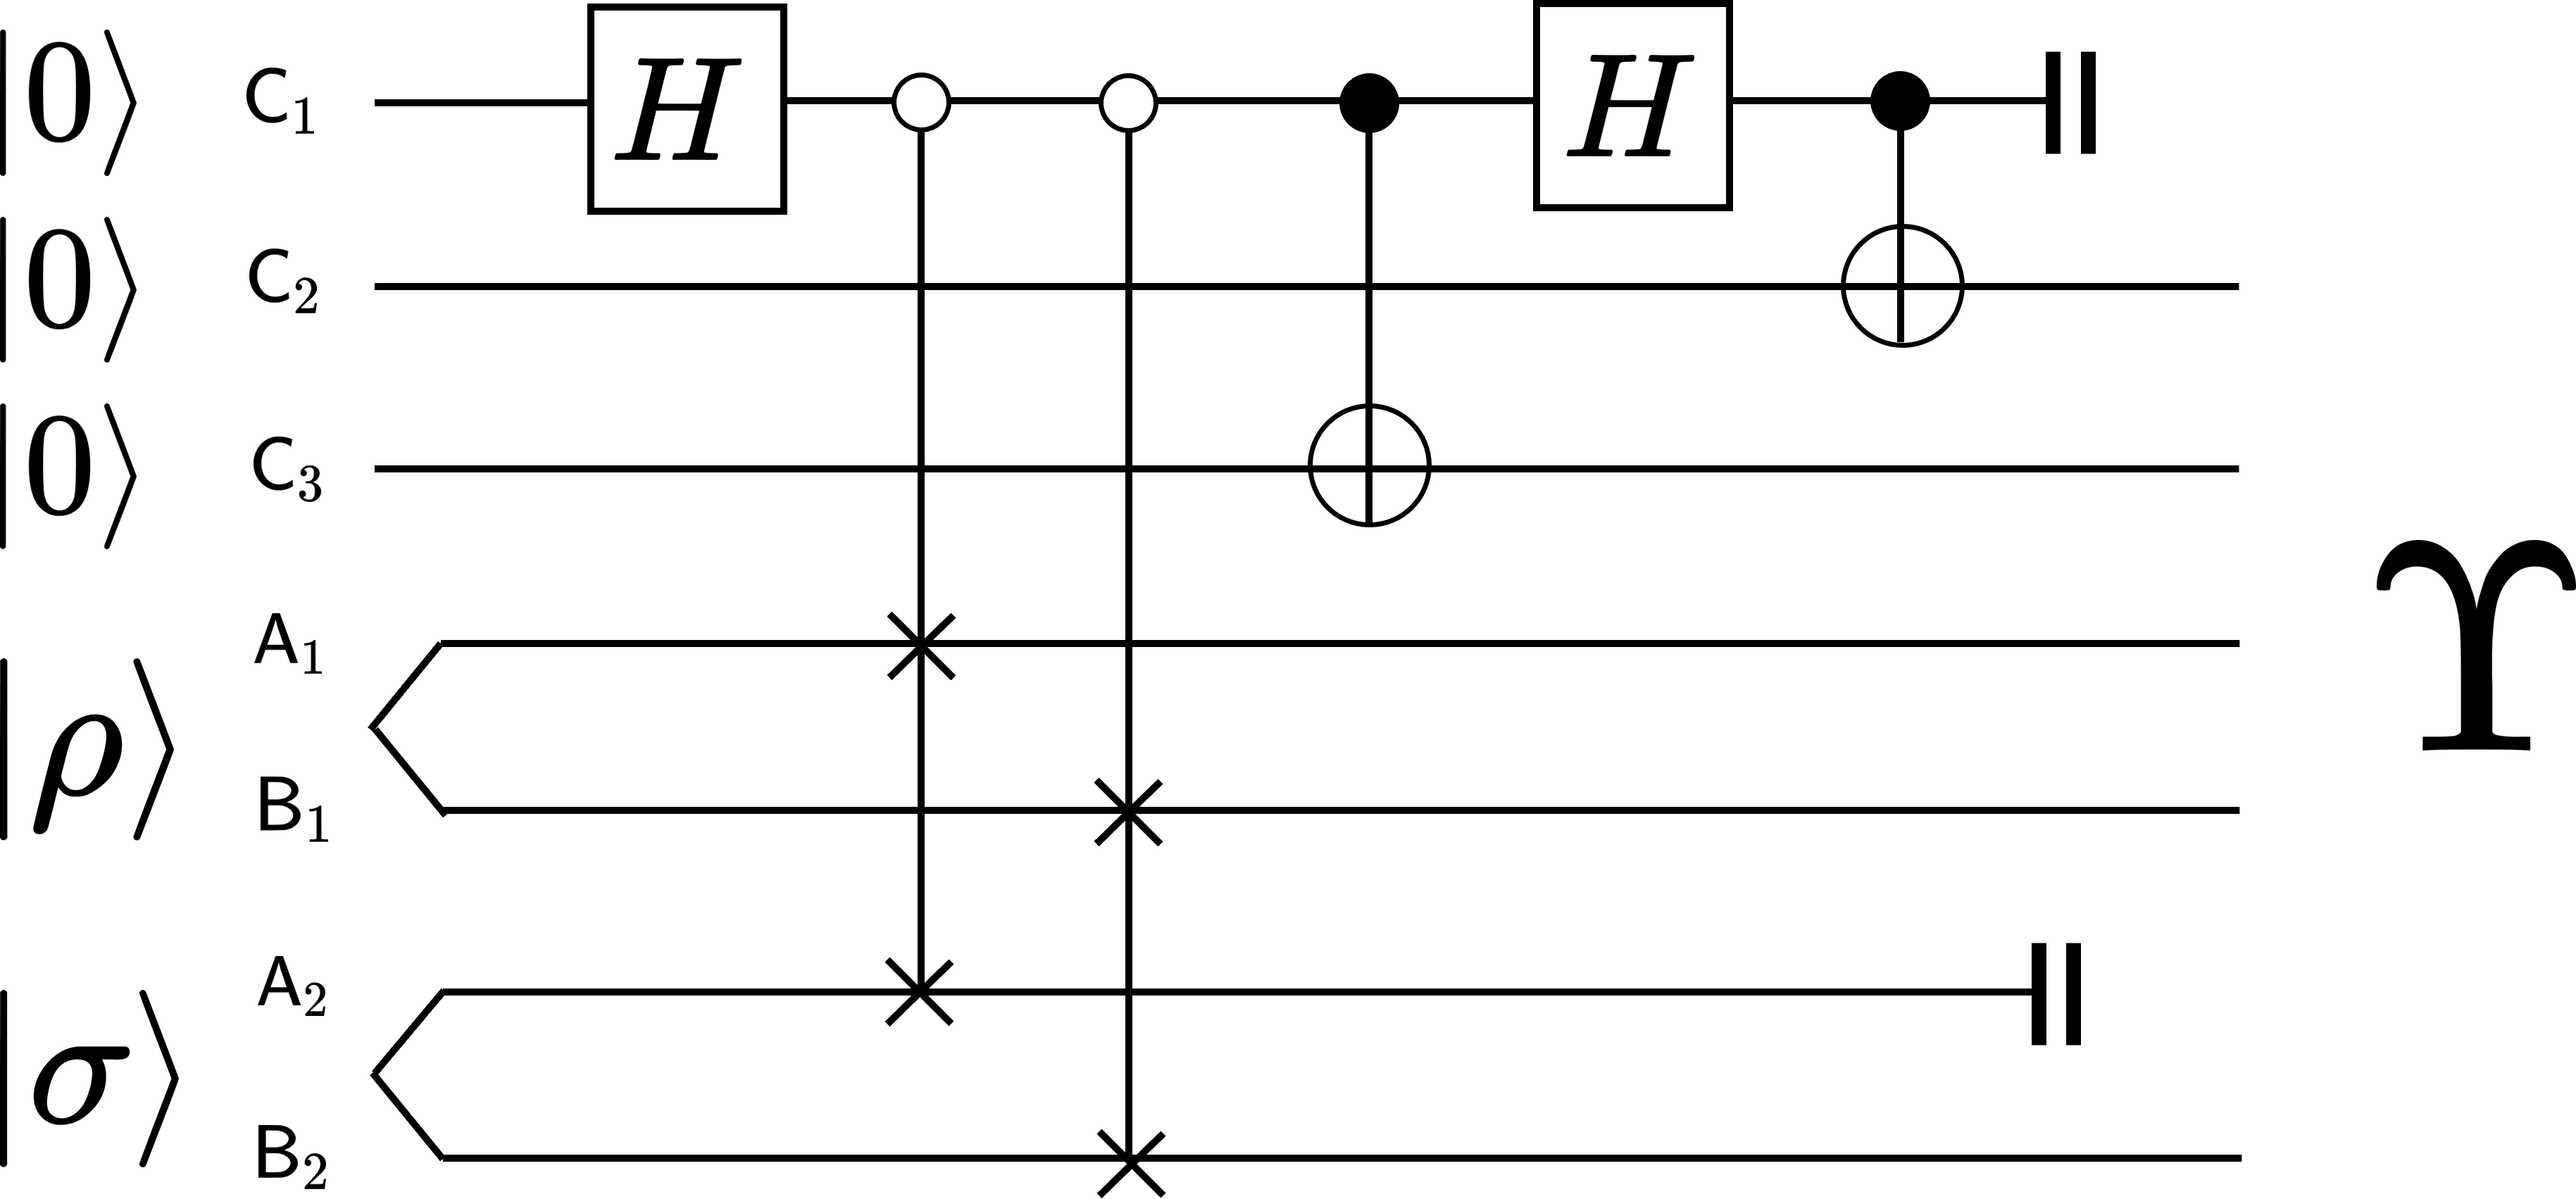
\includegraphics[width=90mm]{fig1.png}
    \caption{A quantum circuit preparing the state $\Upsilon$ in Eq.~\eqref{inteq:64}.
    The systems $\sC_1$, $\sC_2$, and $\sC_3$ are each one-qubit systems. Open circles indicate that the gate is applied when the control qubit is in the state $\ket{0}$, while closed circles indicate control for a qubit in the state $\ket{1}$. The gate $H$ is the one-qubit Hadamard gate. The double vertical lines represent that the qubits of that system are traced out. By convention, the objects with a cross mark and a circle with a cross represent the swap operator and the NOT operator, respectively.}
    \label{fig:upsilon circuit}
\end{figure}














In step 1, we denote by $\Upsilon^{\sC_2\sC_3\sA_1\sB_1\sB_2}$ the output state of the quantum circuit given in \Cref{fig:upsilon circuit}, where each of $\sC_1$, $\sC_2$, and $\sC_3$ is a one-qubit system.
From a direct calculation, we see that $\Upsilon^{\sC_2\sC_3\sA_1\sB_1\sB_2}$ is the form
\begin{align}
\label{inteq:64}
    \Upsilon^{\sC_2\sC_3\sA_1\sB_1\sB_2} 
    = \f{1}{2}\big(\ketbra{0}{0}^{\sC_2} \otimes \xi^{\sC_3\sA_1\sB_1\sB_2} 
    + \ketbra{1}{1}^{\sC_2} \otimes Z^{\sC_3}\xi^{\sC_3\sA_1\sB_1\sB_2} Z^{\sC_3}\big),
\end{align}
where $Z^{\sC_3}$ is the one-qubit Pauli-$Z$ operator acting on $\sC_3$.
The state $\xi^{\sC_3\sA_1\sB_1\sB_2}$ is given by
\begin{align}
    \xi^{\sC_3\sA_1\sB_1\sB_2}
    &= \f{1}{2}\tr_{\sA_2}\big[\big(\ket{0}^{\sC_3}\ket{\sigma}^{\sA_1\sB_1}\ket{\rho}^{\sA_2\sB_2}+\ket{1}^{\sC_3}\ket{\rho}^{\sA_1\sB_1}\ket{\sigma}^{\sA_2\sB_2}\big) \notag \\
    &\hspace{9pc}\big(\bra{0}^{\sC_3}\bra{\sigma}^{\sA_1\sB_1}\bra{\rho}^{\sA_2\sB_2}+\bra{1}^{\sC_3}\bra{\rho}^{\sA_1\sB_1}\bra{\sigma}^{\sA_2\sB_2}\big)\big] \\
    &= \f{1}{2}
\begin{blockarray}{ccc}
& \bra{0}^{\sC_3}&  \bra{1}^{\sC_3} \vspace{1mm}\\
\begin{block}{c(cc)}
  \ket{0}^{\sC_3}\hspace*{1mm} & \ketbra{\sigma}{\sigma}^{\sA_1\sB_1}\otimes\rho^{\sB_2} & \ketbra{\sigma}{\rho}^{\sA_1\sB_1}\otimes (M^{\sB_2})^\dag \\
  \ket{1}^{\sC_3}\hspace*{1mm} & \ketbra{\rho}{\sigma}^{\sA_1\sB_1}\otimes M^{\sB_2} & \ketbra{\rho}{\rho}^{\sA_1\sB_1}\otimes\sigma^{\sB_2} \\
\end{block}
\end{blockarray}\hspace{2.5mm}.
\end{align}
where $M^{\sB_2} = \tr_{\sA_1}\big[\ketbra{\sigma}{\rho}^{\sA_1\sB_2}\big]$.
Since the signs of the off-diagonal entries are flipped by $Z^{\sC_3}$, the state $Z^{\sC_3}\xi^{\sC_3\sA_1\sB_1\sB_2}Z^{\sC_3}$ is given by 
\begin{align}
    Z^{\sC_3}\xi^{\sC_3\sA_1\sB_1\sB_2}Z^{\sC_3}
    = \f{1}{2}
\begin{blockarray}{ccc}
& \bra{0}^{\sC_3}&  \bra{1}^{\sC_3} \vspace{1mm}\\
\begin{block}{c(cc)}
  \ket{0}^{\sC_3}\hspace*{1mm} & \ketbra{\sigma}{\sigma}^{\sA_1\sB_1}\otimes\rho^{\sB_2} & -\ketbra{\sigma}{\rho}^{\sA_1\sB_1}\otimes (M^{\sB_2})^\dag \\
  \ket{1}^{\sC_3}\hspace*{1mm} & -\ketbra{\rho}{\sigma}^{\sA_1\sB_1}\otimes M^{\sB_2} & \ketbra{\rho}{\rho}^{\sA_1\sB_1}\otimes\sigma^{\sB_2} \\
\end{block}
\end{blockarray}\hspace{2mm}.
\end{align}



For step 2, from \Cref{prevthm:DME variant} with $t=2$, we can approximately realize a unitary $e^{iK^{\sC\hat{\sA}\hat{\sB}\sB}}$ within the error $\delta_2$ by using $\mathtt{DMESUB}$ with $m$ copies of $\Upsilon^{\sC_2\sC_3\sA_1\sB_1\sB_2}$, where 
\begin{equation}
\label{eq:m}
m = \Big\lceil\f{16}{\delta_2}\Big\rceil.
\end{equation}
Here, $K^{\sC\hat{\sA}\hat{\sB}\sB}$ is given by
\begin{align}
\label{eq:def of L}
    K^{\sC\hat{\sA}\hat{\sB}\sB} 
    = \xi^{\sC\hat{\sA}\hat{\sB}\sB} - Z^{\sC}\xi^{\sC\hat{\sA}\hat{\sB}\sB}Z^{\sC}
    = 
\begin{blockarray}{ccc}
& \bra{0}^{\sC}&  \bra{1}^{\sC} \vspace{1mm}\\
\begin{block}{c(cc)}
  \ket{0}^{\sC}\hspace*{1.5mm} & 0 & \ketbra{\sigma}{\rho}^{\hat{\sA}\hat{\sB}}\otimes (M^{\sB})^\dag \\
  \ket{1}^{\sC}\hspace*{1.5mm} & \hspace*{0.5mm} \ketbra{\rho}{\sigma}^{\hat{\sA}\hat{\sB}}\otimes M^{\sB} & 0 \\
\end{block}
\end{blockarray}\hspace{2.5mm},
\end{align}
which is an Hermitian matrix with zero diagonal entries.
Although the parameter $t$ can be set to other values, we fix $t = 2$ for simplicity.



Before proceeding to step~3, we examine the structure of the unitary $e^{iK}$. 
For a matrix $A$ with the singular value decomposition $A = \sum_j a_j \ketbra{\eta_j}{\xi_j}$, we define the action of sine and cosine functions on $A$ as
\begin{align}
    &\sin^{(\rm SV)}(A) = \sum_j \sin(a_j)\ketbra{\eta_j}{\xi_j}, \ \ \text{and} \ \ \ \cos^{(\rm SV)}(A) = \sum_j \cos(a_j)\ketbra{\xi_j}{\xi_j}.
\end{align}
Then, the unitary $e^{iK}$ can be rephrased as
\begin{align}
\label{eq:block rep. e^{itK}}
    e^{iK^{\sC\hat{\sA}\hat{\sB}\sB}}
    = \hspace{1mm}
\begin{blockarray}{ccc}
& \bra{0}^{\sC}&  \bra{1}^{\sC} \vspace{1mm}\\
\begin{block}{c(cc)}
  \ket{0}^{\sC}\hspace*{1.5mm} & \cos^{(\rm SV)}(L) & i\sin^{(\rm SV)}(L^\dag) \\
  \ket{1}^{\sC}\hspace*{1.5mm} & i\sin^{(\rm SV)}(L) & \cos^{(\rm SV)}(L^\dag) \\
\end{block}
\end{blockarray}\hspace{2.5mm},
\end{align}
where $L^{\hat{\sA}\hat{\sB}\sB} = \ketbra{\rho}{\sigma}^{\hat{\sA}\hat{\sB}}\otimes M^{\sB}$ and $M^\sB = \tr_{\sA'}\big[\ketbra{\sigma}{\rho}^{\sA'\sB}\big]$.


To see this, let the singular value decomposition of $L^{\hat{\sA}\hat{\sB}\sB}$ be given by $L^{\hat{\sA}\hat{\sB}\sB} = \sum_j s_j \ketbra{l_j}{r_j}^{\hat{\sA}\hat{\sB}\sB}$, and we define $\ket{\psi_j^+}^{\sC\hat{\sA}\hat{\sB}\sB}$ and $\ket{\psi_j^-}^{\sC\hat{\sA}\hat{\sB}\sB}$ by
\begin{align}
    &\ket{\psi_j^+}^{\sC\hat{\sA}\hat{\sB}\sB} = \f{1}{\sqrt{2}}(\ket{0}^\sC \ket{r_j}^{\hat{\sA}\hat{\sB}\sB} + \ket{1}^\sC \ket{l_j}^{\hat{\sA}\hat{\sB}\sB}), \ \ \text{and} \ \ \ \ket{\psi_j^-}^{\hat{\sA}\hat{\sB}\sB} = \f{1}{\sqrt{2}}(\ket{0}^\sC \ket{r_j}^{\hat{\sA}\hat{\sB}\sB} - \ket{1}^\sC \ket{l_j}^{\hat{\sA}\hat{\sB}\sB}).
\end{align}
We can see that these states $\ket{\psi_j^+}^{\sC\hat{\sA}\hat{\sB}\sB}$ and $\ket{\psi_j^-}^{\sC\hat{\sA}\hat{\sB}\sB}$ are eigenstates of $K^{\sC\hat{\sA}\hat{\sB}\sB}$ corresponding eigenvalues $s_j$ and $-s_j$, respectively, because $K^{\sC\hat{\sA}\hat{\sB}\sB}\ket{\psi_j^+}^{\sC\hat{\sA}\hat{\sB}\sB} = s_j \ket{\psi_j^+}^{\sC\hat{\sA}\hat{\sB}\sB}$ and $K^{\sC\hat{\sA}\hat{\sB}\sB}\ket{\psi_j^-}^{\sC\hat{\sA}\hat{\sB}\sB} = -s_j \ket{\psi_j^-}^{\sC\hat{\sA}\hat{\sB}\sB}$~\cite{lloyd2020polardecomposition, lloyd2021hamiltonianQSVT, Lin2022LectureNotes, Odake2024Highoder}.
Thus, $K^{\sC\hat{\sA}\hat{\sB}\sB}$ can be decomposed as $K^{\sC\hat{\sA}\hat{\sB}\sB} = \sum_j \big(s_j\ketbra{\psi_j^+}{\psi_j^+}^{\sC\hat{\sA}\hat{\sB}\sB} - s_j \ketbra{\psi_j^-}{\psi_j^-}^{\sC\hat{\sA}\hat{\sB}\sB} \big)$.
Hence, the unitary $e^{iK}$ can be rewritten as
\begin{align}
    e^{iK}
    &= \sum_j \big(e^{i s_j}\ketbra{\psi_j^+}{\psi_j^+} + e^{-i s_j} \ketbra{\psi_j^-}{\psi_j^-}\big) \\
    &= \sum_j \Big(\f{e^{i s_j}+e^{-i s_j}}{2}\big(\ketbra{0}{0} \otimes \ketbra{r_j}{r_j} 
    + \ketbra{1}{1} \otimes \ketbra{l_j}{l_j}\big) \notag\\
    &\hspace{6pc}+ \f{e^{i s_j}-e^{-i s_j}}{2}\big(\ketbra{0}{1} \otimes \ketbra{r_j}{l_j}
    + \ketbra{1}{0} \otimes \ketbra{l_j}{r_j}\big)\Big) \\
    &= \ketbra{0}{0} \otimes \cos^{(\rm SV)}(L) + \ketbra{1}{1} \otimes \cos^{(\rm SV)}(L^\dag) \notag\\
    &\hspace{6pc}+ \ketbra{0}{1} \otimes i\sin^{(\rm SV)}(L^\dag) + \ketbra{1}{0} \otimes i\sin^{(\rm SV)}(L).
\end{align}





Let $U_2^{\sC\hat{\sA}\hat{\sB}\sB} = -iX^\sC e^{iK^{\sC\hat{\sA}\hat{\sB}\sB}}$, where $X^\sC$ is the one-qubit Pauli-$X$ gate on the system $\sC$. Since $e^{iK^{\sC\hat{\sA}\hat{\sB}\sB}}$ is given in Eq.~\eqref{eq:block rep. e^{itK}}, we see that $U_2^{\sC\hat{\sA}\hat{\sB}\sB}$ is a block-encoding unitary of $\sin^{(\rm SV)}(L^{\hat{\sA}\hat{\sB}\sB}) = \ketbra{\rho}{\sigma}^{\hat{\sA}\hat{\sB}} \otimes \sin^{(\rm SV)}(M^\sB)$:
\begin{align}
    U_2^{\sC\hat{\sA}\hat{\sB}\sB}
    &= \hspace{1mm}
\begin{blockarray}{ccc}
& \bra{0}^\sC &  \vspace{1mm}\\
\begin{block}{c(cc)}
  \ket{0}^\sC \hspace*{1mm} & \ketbra{\rho}{\sigma}^{\hat{\sA}\hat{\sB}}\otimes \sin^{(\rm SV)}\big(M^\sB\big) & \hspace{0mm} * \hspace{3mm}\\
  & * & \hspace{0mm} * \hspace{3mm}\\
\end{block}
\end{blockarray}\hspace{2.5mm}.
\end{align}
The term $\ketbra{\sigma}{\rho}^{\hat{\sA}\hat{\sB}}$ is irrelevant to the singular values.
Although the coefficient $-i$ is clearly not essential since $-iX(\cdot)(-iX)^\dag = X(\cdot)X$, it is introduced here for simplicity.
Noting that the diamond norm is invariant under unitaries, we can obtain a quantum channel $\cG^{\sC\hat{\sA}\hat{\sB}\sB}$ that satisfies
\begin{equation}
\label{eq:matrix exponentiation of M}
    \f{1}{2}\|\cG^{\sC\hat{\sA}\hat{\sB}\sB} - \cU_2^{\sC\hat{\sA}\hat{\sB}\sB}\|_\diamond \leq \delta_2,
\end{equation}
by $\mathtt{DMESUB}(\Upsilon^{\sC_2\sC_3\sA_1\sB_1\sB_2}; \delta_2, t=2)$.


By using $\mathtt{DMESUB}^\dag$ instead of $\mathtt{DMESUB}$, we can approximate $e^{-iK^{\sC\hat{\sA}\hat{\sB}\sB}}$ from $\Upsilon^{\sC_2\sC_3\sA_1\sB_1\sB_2}$, and hence approximate $(U_2^{\sC\hat{\sA}\hat{\sB}\sB})^\dag = ie^{-iK^{\sC\hat{\sA}\hat{\sB}\sB}} X^\sC$. That is, we can obtain a quantum channel $\cG_{\rm inv}^{\sC\hat{\sA}\hat{\sB}\sB}$ such that
\begin{align}
\label{inteq:92}
    \f{1}{2}\big\|\cG_{\rm inv}^{\sC\hat{\sA}\hat{\sB}\sB} - (\cU_2^{\sC\hat{\sA}\hat{\sB}\sB})^\dag\big\|_\diamond \leq \delta_2,    
\end{align}
using $\mathtt{DMESUB}^\dag$ that takes the same number of samples and gates as $\mathtt{DMESUB}$.


Since $M^\sB = \tr_{\sA'}\big[\ketbra{\sigma}{\rho}^{\sA'\sB}\big]$, we obtain $\ketbra{\rho}{\sigma}^{\hat{\sA}\hat{\sB}} \otimes V^\sB$ by lifting up all the singular values of $\ketbra{\rho}{\sigma}^{\hat{\sA}\hat{\sB}}\otimes \sin^{(\rm SV)}\big(M^\sB\big)$ to unity, where $V^\sB$ is the Uhlmann partial isometry (see also \Cref{prop:explicit form of Uhl}).
To achieve that, we use the QSVT with the sign function in step 3.


Using $\mathtt{QSVTSIGN}$ in \Cref{prop:FPAA general} with input $\cG^{\sC\hat{\sA}\hat{\sB}\sB}$ and $\cG_{\rm inv}^{\sC\hat{\sA}\hat{\sB}\sB}$, we can realize a quantum channel $\cJ^{\sB\sH\hat{\sA}\hat{\sB}}$ that satisfies
\begin{equation}
\label{inteq:16}
    \f{1}{2}\big\|\cJ^{\sB\sH\hat{\sA}\hat{\sB}} - \cU_1^{\sB\sH\hat{\sA}\hat{\sB}}\big\|_\diamond \leq u\delta_2,
\end{equation}
where $\sH$ is a two-qubit system and $u$ is the minimum odd integer such that 
\begin{align} 
\label{eq:u} 
    u \geq \Big\lceil \f{8 e}{\beta}\log{\Big(\f{2}{\delta_1}\Big)} \Big\rceil.
\end{align}
The unitary $U_1^{\sH\hat{\sA}\hat{\sB}\sH}$ is given by
\begin{align}
\label{inteq:61}
    U_1^{\sB\sH\hat{\sA}\hat{\sB}} 
    = \hspace{1mm}
\begin{blockarray}{ccc}
& \bra{0^2}^\sH&  \vspace{1mm}\\
\begin{block}{c(cc)}
  \ket{0^2}^\sH \hspace*{1mm} & \ketbra{\rho}{\sigma}^{\hat{\sA}\hat{\sB}}\otimes P_\sgn^{(\rm SV)}\big(\sin^{(\rm SV)}(M^\sB)\big) & \hspace{0mm} * \hspace{3mm}\\
  & * & \hspace{0mm} * \hspace{3mm}\\
\end{block}
\end{blockarray}\hspace{2.5mm},
\end{align}
where $P_\sgn$ satisfies $|P_\sgn(x) - \sgn(x)| \leq \delta_1$ for $x \in [\beta, 1]$.
This follows from replacing $U_2^{\sC\hat{\sA}\hat{\sB}\sB}$ and $(U_2^{\sC\hat{\sA}\hat{\sB}\sB})^\dag$, used a total of $u$ times in the quantum circuit for $\mathtt{QSVTSIGN}$, with a channel $\cG^{\sC\hat{\sA}\hat{\sB}\sB}$ and $\cG_{\rm inv}^{\sC\hat{\sA}\hat{\sB}\sB}$, respectively, which approximate these unitaries as Eqs.~\eqref{eq:matrix exponentiation of M} and~\eqref{inteq:92}.
The overall error is evaluated using the subadditivity of the diamond norm.
Note that
\begin{align}
    P_\sgn^{(\rm SV)}\big(\ketbra{\sigma}{\rho}^{\hat{\sA}\hat{\sB}} \otimes \sin^{(\rm SV)}(M^\sB)\big)
    = \ketbra{\sigma}{\rho}^{\hat{\sA}\hat{\sB}} \otimes P_\sgn^{(\rm SV)}\big(\sin^{(\rm SV)}(M^\sB)\big).
\end{align}




The discussion so far is applicable to both cases, where the performance of our algorithm is measured by either the diamond norm or the fidelity difference.
In the following, we evaluate these two cases separately.
In \Cref{sec:FPAA part}, we provide a proof with the approximation error measured by the diamond norm, while in \Cref{sec:uhlfidquery}, we focus on the fidelity difference, which leads to fewer samples.
These results give the full statement of Theorem~\ref{thm:algorithm Uhlmann}.





%=============================================================================================================================================================================
%=============================================================================================================================================================================





\subsubsection{Evaluation in the diamond norm}
\label{sec:FPAA part}


We evaluate a distance between $U_1^{\sB\sH\hat{\sA}\hat{\sB}}$ and a unitary $U_{\rm ideal}^{\sB\sH}$ which is an exact block-encoding of $\ketbra{\rho}{\sigma}^{\hat{\sA}\hat{\sB}}\otimes\sgn^{(\rm SV)}\big(\sin^{(\rm SV)}(M^\sB)\big)$:
\begin{align}
    U_{\rm ideal}^{\sB\sH\hat{\sA}\hat{\sB}} 
    = \hspace{1mm}
\begin{blockarray}{ccc}
& \bra{0^2}^\sH&  \vspace{1mm}\\
\begin{block}{c(cc)}
  \ket{0^2}^\sH \hspace*{1mm} & \ketbra{\rho}{\sigma}^{\hat{\sA}\hat{\sB}}\otimes \sgn^{(\rm SV)}\big(\sin^{(\rm SV)}(M^\sB)\big) & \hspace{0mm} * \hspace{3mm}\\
  & * & \hspace{0mm} * \hspace{3mm}\\
\end{block}
\end{blockarray}\hspace{2.5mm}.
\end{align}
We note that $\sgn^{(\rm SV)}\big(\sin^{(\rm SV)}(M^\sB)\big)$ corresponds to the Uhlmann partial isometry $V^\sB$ because the singular values of $M^\sB$ correspond to those of $\sqrt{\sigma^\sA}\sqrt{\rho^\sA}$, hence all lie within $[0, 1]$, and in $x \in [0, 1]$, $0 \leq \sin(x) \leq 1$. 

The function $\sin(x)$ increases monotonically in $x \in [0, 1]$ and satisfies $\f{2}{\pi} x \leq \sin(x)$.
Thus, by setting $\beta$ as $\beta = \beta_\diamond = \f{2}{\pi}s_{\rm min}$, where $s_{\min}$ is the minimum non-zero singular value of $\sqrt{\sigma^\sA}\sqrt{\rho^\sA}$, from \Cref{prop:FPAA general}, we have that
\begin{align}
\label{inteq:89}
    \big\|P_\sgn^{(\rm SV)}\big(\sin^{(\rm SV)}(M^\sB)\big) - \sgn^{(\rm SV)}\big(\sin^{(\rm SV)}(M^\sB)\big)\big\|_\infty \leq \delta_1.
\end{align}
From \Cref{lem:FPAA diamond}, when Eq.~\eqref{inteq:89} holds, we obtain that
\begin{align}
\label{inteq:25}
    \f{1}{2}\big\|\cU_1^{\sB\sH\hat{\sA}\hat{\sB}}\circ\cP_{\ket{0}\ket{\sigma}}^{\bC\rarr\sH\hat{\sA}\hat{\sB}} - \cU_{\rm ideal}^{\sB\sH\hat{\sA}\hat{\sB}}\circ\cP_{\ket{0}\ket{\sigma}}^{\bC\rarr\sH\hat{\sA}\hat{\sB}}\big\|_\diamond \leq 3\sqrt{\delta_1},
\end{align}
where $\cP_{\ket{0}\ket{\sigma}}^{\bC\rarr\sH\hat{\sA}\hat{\sB}} = \ketbra{0^2}{0^2}^\sH \otimes \ketbra{\sigma}{\sigma}^{\hat{\sA}\hat{\sB}}$.
Note that, in the purified sample access model, we can easily implement the channel $\cP_{\ket{\sigma}}^{\bC\rarr\hat{\sA}\hat{\sB}}$, since it only involves assigning one of the given copies of $\ket{\sigma}^{\hat{\sA}\hat{\sB}}$.



Finally, we evaluate the total error of the whole algorithm using the triangle inequality. 
We can evaluate the error as
\begin{align}
    \big\|\cJ^{\sB\sH\hat{\sA}\hat{\sB}}\circ\cP_{\ket{0}\ket{\sigma}}^{\bC\rarr\sH\hat{\sA}\hat{\sB}} - \cU_{\rm ideal}^{\sB\sH\hat{\sA}\hat{\sB}}\circ\cP_{\ket{0}\ket{\sigma}}^{\bC\rarr\sH\hat{\sA}\hat{\sB}}\big\|_\diamond  
    &\leq \big\|\cJ^{\sB\sH\hat{\sA}\hat{\sB}}\circ\cP_{\ket{0}\ket{\sigma}}^{\bC\rarr\sH\hat{\sA}\hat{\sB}} - \cU_1^{\sB\sH\hat{\sA}\hat{\sB}}\circ\cP_{\ket{0}\ket{\sigma}}^{\bC\rarr\sH\hat{\sA}\hat{\sB}}\big\|_\diamond     \notag\\
    &\hspace{3pc}+ \big\|\cU_1^{\sB\sH\hat{\sA}\hat{\sB}}\circ\cP_{\ket{0}\ket{\sigma}}^{\bC\rarr\sH\hat{\sA}\hat{\sB}} - \cU_{\rm ideal}^{\sB\sH\hat{\sA}\hat{\sB}}\circ\cP_{\ket{0}\ket{\sigma}}^{\bC\rarr\sH\hat{\sA}\hat{\sB}}\big\|_\diamond \\
    &\leq \big\|\cJ^{\sB\sH\hat{\sA}\hat{\sB}} - \cU_1^{\sB\sH\hat{\sA}\hat{\sB}}\big\|_\diamond \big\|\cP_{\ket{0}\ket{\sigma}}^{\bC\rarr\sH\hat{\sA}\hat{\sB}}\big\|_\diamond    \notag\\
    &\hspace{3pc}+ \big\|\cU_1^{\sB\sH\hat{\sA}\hat{\sB}}\circ\cP_{\ket{0}\ket{\sigma}}^{\bC\rarr\sH\hat{\sA}\hat{\sB}} - \cU_{\rm ideal}^{\sB\sH\hat{\sA}\hat{\sB}}\circ\cP_{\ket{0}\ket{\sigma}}^{\bC\rarr\sH\hat{\sA}\hat{\sB}}\big\|_\diamond.
\end{align}
Thus, as $\big\|\cP_{\ket{0}\ket{\sigma}}^{\bC\rarr\sH\hat{\sA}\hat{\sB}}\big\|_\diamond = 1$, and from Eqs.~\eqref{inteq:16} and~\eqref{inteq:25}, we obtain that, for $\delta_2 \in (0, 1)$ and $\delta_1 \in (0, 1/2)$,
\begin{align}
\label{inteq:103}
    \f{1}{2} \big\|\cJ^{\sB\sH\hat{\sA}\hat{\sB}}\circ\cP_{\ket{0}\ket{\sigma}}^{\bC\rarr\sH\hat{\sA}\hat{\sB}} - \cU_{\rm ideal}^{\sB\sH\hat{\sA}\hat{\sB}}\circ\cP_{\ket{0}\ket{\sigma}}^{\bC\rarr\sH\hat{\sA}\hat{\sB}}\big\|_\diamond
    \leq 3\sqrt{\delta_1} + u\delta_2.
\end{align}
By rescaling these parameters, such as $\delta_1 = (\delta/6)^2$ and $\delta_2 = \delta/(2u)$, the overall error is bounded by $\delta$.


The number of samples $w_\diamond = um$ of $\ket{\rho}^{\hat{\sA}\hat{\sB}}$ and $\ket{\sigma}^{\hat{\sA}\hat{\sB}}$ is given by 
\begin{align}
    w_\diamond 
    &= \cO\Big(\f{1}{\delta_2 \beta_\diamond}\log{\Big(\f{1}{\delta_1}\Big)}\Big) \\
    &= \cO\Big(\f{1}{\delta s_{\rm min}^2}\Big(\log{\Big(\f{1}{\delta}\Big)}\Big)^2\Big),
\end{align}
where $u$ is the minimum odd integers satisfying Eq.~\eqref{eq:u} and $m$ is given by Eq.~\eqref{eq:m}, while we set $\beta = \beta_\diamond = 2 s_{\rm min}/\pi$.


The quantum circuit in \Cref{fig:upsilon circuit} involves a constant number of one- and two-qubit gates, as well as a controlled-swap operation acting on $\log{(d_\sA d_\sB)}$ qubits, which can be implemented using $\cO\big(\log{(d_\sA d_\sB)}\big)$ gates. The entire algorithm consists of $\cO(w_\diamond)$ applications of this circuit.
Hence, the quantum circuit of the algorithm involves $\cO\big(w\log{(d_\sA d_\sB)}\big)$ one- and two-qubit gates.
Note that, although it might be expected that $\cO\big(w_\diamond\log{(d_\sA d_\sB)}\big)$ auxiliary qubits are required, in fact, $\cO\big(\log{(d_\sA d_\sB)}\big)$ qubits suffice at any time, since this algorithm is carried out sequentially.
This qubits includes those for storing the samples of $\ket{\rho}^{\hat{\sA}\hat{\sB}}$ and $\ket{\sigma}^{\hat{\sA}\hat{\sB}}$, and the constant number of additional qubits.












%============================================================================================================================================================





\subsubsection{Evaluation in the fidelity difference}
\label{sec:uhlfidpurifsamp}


When we evaluate the error using the fidelity difference, 
\begin{align}
    \rF(\rho^\sA, \sigma^\sA) - \rF(\cT^\sB(\ketbra{\rho}{\rho}^{\sA\sB}), \ket{\sigma}^{\sA\sB}),
\end{align}
the sample complexity of the Uhlmann transformation could be smaller than $\cO\Big(\big(\log{(1/\delta)}\big)^2/(\delta s_{\rm min}^2)\Big)$ derived in the previous section.
To show this, we modify only the part of step~3 corresponding to the QSVT with the sign function.




First, we consider the difference between 
\begin{align}
    \sqrt{\rF} 
    = \sqrt{\rF}(\rho^\sA, \sigma^\sA)
    = \sqrt{\rF}(V^\sB\ket{\rho}^{\sA\sB}, \ket{\sigma}^{\sA\sB}), \ \ \ \textrm{and} \ \ \ 
    \sqrt{\rF'} 
    = \sqrt{\rF}(U_1^{\sB\sH\hat{\sA}\hat{\sB}}\ket{\rho}^{\sA\sB}\ket{0^2}^\sH\ket{\sigma}^{\hat{\sA}\hat{\sB}}, \ket{\sigma}^{\sA\sB}\ket{0^2}^\sH\ket{\rho}^{\hat{\sA}\hat{\sB}}).
\end{align}
Remember that $V^\sB$ is the Uhlmann partial isometry, $U_1^{\sB\sH\hat{\sA}\hat{\sB}}$ is a block-encoding unitary of $\ketbra{\rho}{\sigma}^{\hat{\sA}\hat{\sB}} \otimes P_\sgn^{(\rm SV)}\big(\sin^{(\rm SV)}(M^\sB)\big)$ (see Eq.~\eqref{inteq:61}), and $M^\sB = \tr_{\sA'}[\ketbra{\sigma}{\rho}^{\sA'\sB}]$.


As the similar calculation in \Cref{sec:uhlfidquery}, we see that
\begin{align}
\label{inteq:120}
    \big|\sqrt{\rF} - \sqrt{\rF'}\big|
    &= \big| |\bra{\sigma}V^\sB\ket{\rho}^{\sA\sB}| - |\bra{\sigma}P_\sgn^{(\rm SV)}\big(\sin^{(\rm SV)}(M)^\sB\big)\ket{\rho}^{\sA\sB}| \big| \\
    &\leq \sum_k \big|1 - P_\sgn\big(\sin(s_k)\big)\big|s_k \notag\\
    \label{inteq:40}
    &= \sum_{k\in I_\beta} \big|1 - P_\sgn\big(\sin(s_k)\big)\big|s_k  + \sum_{k\in \bar{I}_\beta} \big|1 - P_\sgn\big(\sin(s_k)\big)\big|s_k \\
    &\leq \delta_1 + 2 \sum_{k\in \bar{I}_\beta} s_k \\
    &\leq \delta_1 +  \pi\beta r,
\end{align}
where $I_\beta = \{k \in \bN; \beta \leq \sin(s_k)\}$, $\bar{I}_\beta = \{k \in \bN; \beta > \sin(s_k)\}$, and $r$ is the rank of $\sqrt{\sigma^\sA}\sqrt{\rho^\sA}$.
In the last inequality, we use $s_k \leq \f{\pi}{2}\sin(s_k) < \f{\pi}{2}\beta$ for $k \in \bar{I}_\beta$ and $\#\bar{I}_\beta = \sum_{k \in \bar{I}_\beta} 1 \leq r$.



Thus, setting $\beta$ as $1/\beta = \pi r/\delta_1$ ensures $\big|\sqrt{\rF} - \sqrt{\rF'}\big| \leq 2\delta_1$. 
On the other hand, if we choose $1/\beta = \pi/(2s_{\rm min})$, $\bar{I}_\beta$ is empty, which leads to $\big|\sqrt{\rF} - \sqrt{\rF'}\big|\leq \delta_1$.
Hence, $\beta$ is chosen as $\beta = \beta_\tF$, where $1/\beta_\tF = \pi\min\{1/(2s_{\rm min}), r/\delta_1\}$, 
to ensure that 
\begin{align}
\label{inteq:51}
    \big|\sqrt{\rF} - \sqrt{\rF'}| \leq 2\delta_1.
\end{align}
Using that $|x-y|\leq 2|\sqrt{x}-\sqrt{y}|$ for $0\leq x, y \leq 1$, we obtain $\big|\rF - \rF'| \leq 4\delta_1$.

Next, we define $\rF''$ by 
\begin{align}
    \rF'' = \rF\big(\cJ^{\sB\sH\hat{\sA}\hat{\sB}}\circ\cP_{\ket{0}\ket{\sigma}}^{\bC\rarr\sH\hat{\sA}\hat{\sB}}(\ketbra{\rho}{\rho}^{\sA\sB}), \ket{\sigma}^{\sA\sB}\ket{0^2}^\sH\ket{\rho}^{\hat{\sA}\hat{\sB}}\big).
\end{align} 
Then, the difference between $\rF''$ and $\rF$ can be calculated as
\begin{align}
    \big|\rF'' - \rF\big| 
    &\leq \big|\rF'' - \rF'\big| + \big|\rF' - \rF\big| \\
    &\leq\big|\rF'' - \rF'\big| + 4\delta_1 \\
    &\leq \f{1}{2}\big\|\cJ^{\sB\sH\hat{\sA}\hat{\sB}} - \cU_1^{\sB\sH\hat{\sA}\hat{\sB}} \big\|_\diamond + 4\delta_1 \\
    \label{inteq:106}
    &\leq u\delta_2 + 4\delta_1,
\end{align}
where $u$ is given by the minimum odd integer satisfying $u \geq \big\lceil\f{8e}{\beta_\tF}\log{(2/\delta_1)}\big\rceil$.
In the third inequality, we used the relation between the diamond norm and the fidelity Eq.~\eqref{eq:fidelity and diamond} and $\|\cP_{\ket{0}\ket{\sigma}}^{\bC\rarr\sH\hat{\sA}\hat{\sB}}\|_\diamond = 1$.
We also used Eq.~\eqref{inteq:16} in the last inequality.



By rescaling these parameters, such as $\delta_1 = \delta/8$ and $\delta_2 = \delta/(2u)$, and defining $\cT^\sB$ by $\cT^\sB = \tr_{\sH\hat{\sA}\hat{\sB}}\circ\cJ^{\sB\sH\hat{\sA}\hat{\sB}}\circ\cP_{\ket{0}\ket{\sigma}}^{\bC\rarr\sH\hat{\sA}\hat{\sB}}$, we obtain that
\begin{align}
    \rF\big(\cT^\sB(\ketbra{\rho}{\rho}^{\sA\sB}), \ket{\sigma}^{\sA\sB}\big)
    \geq \rF(\rho^\sA, \sigma^\sA) - \delta,
\end{align}
which follows from the fact that $\rF(\rho^\sA, \sigma^\sA) \geq \rF\big(\cT^\sB(\ketbra{\rho}{\rho}^{\sA\sB}), \ket{\sigma}^{\sA\sB}\big)$.
The number of samples $w_\tF = um$ of the states $\ket{\rho}^{\hat{\sA}\hat{\sB}}$ and $\ket{\sigma}^{\hat{\sA}\hat{\sB}}$ is given by
\begin{align}
    w_\tF &= \cO\Big(\f{1}{\delta_2\beta_\tF}\log{\Big(\f{1}{\delta_1}\Big)}\Big) \\
    &= \cO\Big(\f{1}{\delta}\min\Big\{\f{1}{s_{\rm min}^2}, \f{r^2}{\delta^2}\Big\}\Big(\log{\Big(\f{1}{\delta}\Big)}\Big)^2\Big).
\end{align}
The circuit of the algorithm consists of
$\cO\big(w_\tF \log{(d_\sA d_\sB)}\big)$ one- and two-qubit gates, and $\cO(\log{(d_\sA d_\sB)})$ qubits suffice at any one time.
We completed the proof of Theorem~\ref{thm:algorithm Uhlmann}.



%====================================================================================================================================
